%
% versuch.tex -- Paper zum Thema Optische Fouriertransformation <opt>
%
% (c) 2023 Marco Niederberger, Yanick Schoch; OST Ostschweizer Fachhochschule
%
% !TEX root = ../../buch.tex
% !TEX encoding = UTF-8
%
\section{Versuch
  \label{opt:section:versuch}}
\rhead{Praktische Erprobung}

Der durchgeführte Versuch entspricht im Aufbau demjenigen aus Abbildung \ref{opt:fig:4fAufbau}.
Als Linsen für die Fouriertransformation wurden eine mit 300 mm Brennweite genutzt, damit der Effekt am besten sichtbar war.
Um die gerade Wellenfront in ausreichendem Durchmesser zu erhalten, wurde der Laser mittels eines umgekehrten keplerschen Teleskops aufgeweitet.
Der schematische Aufbau ist in Abbildung \ref{opt:fig:laserAufweiten} ersichtlich.
Dafür wird direkt hinter der Laserblende eine konkave Linse mit einer Brennweite $f_b = 50\,\text{mm}$ montiert 
und in einem Abstand von $f_b + f_o = 200\,\text{mm}$ eine weitere mit einer Brennweite von $f_o = 150\,\text{mm}$.
Somit wird der Laserstrahl um ein Faktor $\frac{f_o}{f_b} = 3$ vergrössert.
Dies war ausreichend, um die vorhandenen Blenden vollständig auszuleuchten.

Nachdem der Laserstrahl vorbereitet wurde, wird eine erste Blende montiert.
In Abbildung \ref{opt:fig:4fAufbau} ist dies als Originalbild beschrieben.
Im Abstand $f=300\,\text{mm}$ wird jetzt die erste Linse montiert und nach weiteren zwei Brennweiten die zweite Linse.
Genau in der Mitte der beiden Linsen ergibt sich die Fourierebene.
Ganz am Ende des Aufbaus, eine weitere Brennweite hinter der zweiten Linse ist das rücktransformierte Bild ersichtlich.

Im weiteren Verlauf dieses Kapitels werden die erwarteten Ergebnisse simuliert und anschliessend mit den Beobachtungen verglichen.

\subsection{Simulation der erwarteten Ergebnissen}
Der $4f$ Versuch kann auch simuliert werden.
In unserem Fall geschah dies mit \emph{Python} und der \emph{numpy} Bibliothek.
In einem ersten Schritt wird ein Input-Bild erstellt, auf welchem eine oder mehrere Gitter ersichtlich sind.
Mittels zweidimensionaler diskreter Fouriertransformation wird das Originalbild in den Frequenzbereich transformiert.
Anschliessend kann dies mit einem digitalen Filter gefiltert werden.
Die Filter werden so ausgeführt, wie sie in Abbildung \ref{opt:fig:filterarten} aufgeführt sind.
Das bedeutet, dass zum Beispiel ein Tiefpass einen runden Durchlassbereich um den Nullpunkt hat.
Schlussendlich wird das gefilterte Frequenzspektrum mittels zweidimensionaler FFT wieder rücktransformiert.

\subsection{Versuchsdurchführung}
Zuerst wurde die Funktion des Aufbaus mit einem $2f$ Versuch verifiziert.
Dabei wird nur eine Linse aus dem $4f$ Aufbau verwendet und das entstandene Spektrum wird im Abstand der Brennweite betrachtet.
Die dabei entstandenen Bilder entsprachen den Erwartungen.
Für den Einzelspalt war, wie in Abschnitt \ref{opt:sec:exampleSingleSlit} berechnet, eine sinc-förmige Verteilung der Intensität zu betrachten.

Nach dieser Verifizierung wurde die zweite Linse ebenfalls montiert und die Abbildungsebene hinter die zweite Linse gelegt.
Beim Dreifachspalt konnte die Fouriertransformation und Rücktransformation erfolgreich ausgeführt werden.
Die Filterung mittels eines optischen Tiefpasses konnte jedoch nicht nachgebildet werden.
Der genaue Grund dafür konnte nicht eruiert werden.
Mögliche Ursachen wären eine zu grosse Blende, eine nicht optimale Ausrichtung der optischen Achse oder eine zu geringe Auflösung der Auswerteeinheit.


\subsection{Vergleich der Simulation}

\begin{figure}
    \centering
    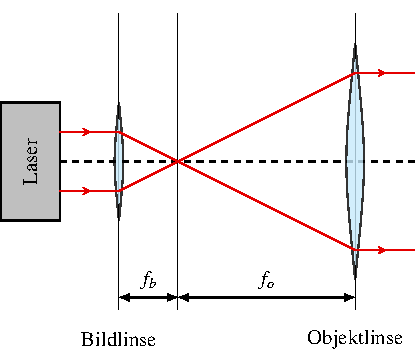
\includegraphics[width=60mm]{papers/opt/images/laserAufweiten.pdf}
    \caption{Die Vergrösserung des Laserlichts erfolgt mit einem Kepler-Teleskop.
        Dazu werden zwei Linsen mit unterschiedlichen Brennweiten verwendet.
        Der Abstand dazwischen ist die Summe der beiden Brennweiten.}
    \label{opt:fig:laserAufweiten}
\end{figure}

\begin{figure}
    \centering
    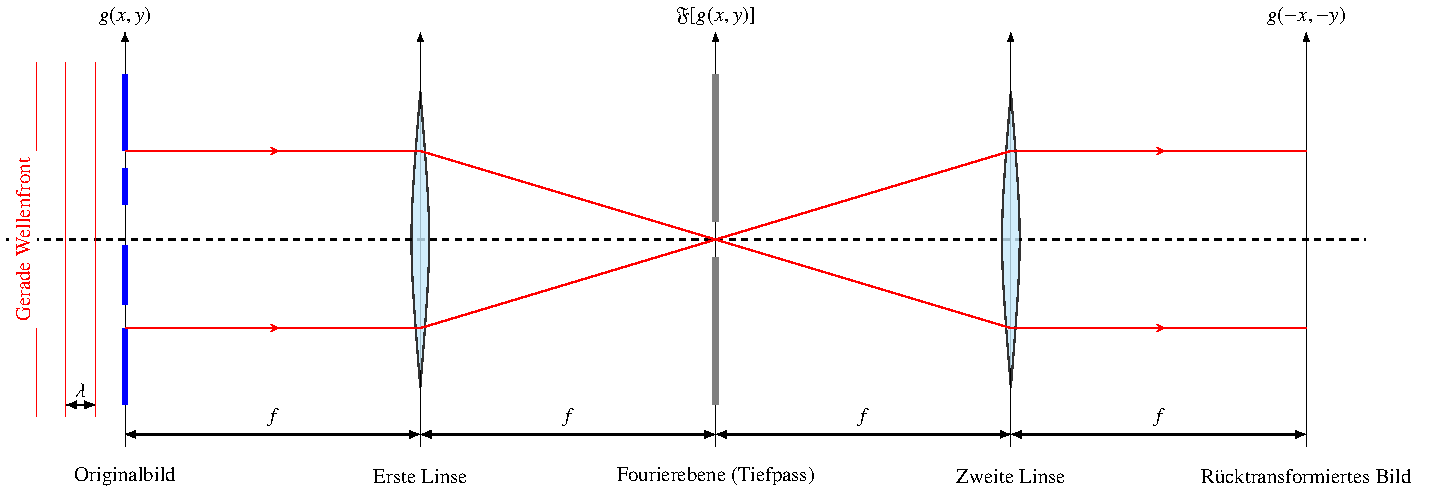
\includegraphics[width=\textwidth]{papers/opt/images/4fAufbau.pdf}
    \caption{Der $4f$ Aufbau ermöglicht eine Fouriertransformation des Originalbildes sowie eine Rücktransformation aus der Fourierebene.
    In dieser Abbildung wird die transformierte Funktion mit einem Tiefpass gefiltert.
    Weitere Details zu den Filtern folgen im Kapitel \ref{opt:section:filter}.}
    \label{opt:fig:4fAufbau}
\end{figure}
